%!TEX root = ../tesis_mbc.tex

\chapter{Introducción}
\label{ch:intro}

\begin{chapterquote}{Chris Anderson}
	A Long Tail is just culture  unfiltered by economic scarcity.
\end{chapterquote}

\section{Motivación}

Con la cantidad de información que se genera hoy en día y la cantidad de servicios \textit{online} que tenemos, para explotar el fenómeno conocido como \textit{long tail} en \textit{marketing} los proveedores de estos servicios quieren personalizar el contenido que ofrecen a sus usuarios; en particular quieren predecir la respuesta del usuario a distintas opciones. A este tipo de sistemas se les conoce como \textbf{sistemas de recomendación}, y tal vez el más conocido es el de \textit{Netflix}; sin embargo, existen más, como la sección de 'Qué ver' en \textit{YouTube} o los destinos que nos recomiendan en \textit{Airbnb} o lo productos que nos recomiendan en \textit{Amazon}.

Los sistemas de recomendación se han vuelto más populares últimamente por varias razones, pero todo se podría resumir en un solo concepto: \textit{long tail} o cola larga. Este concepto rompe la creencia del principio de Pareto que afirma que el 80\% de las consecuencias (ganancias) provienen del 20\% de las causas (productos). Este principio se ha usado como regla de dedo en distintas disciplinas, pero en ciertos productos no se cumple, por ejemplo, las rentas de películas en \textit{Netflix}, las cuales tienen una cola larga. En una distribución de cola larga, es menos del 80\% de las ganancias el que proviene del 20\% de los productos, esto significa que se pueden tener ganancias a partir de productos no tan populares. Se puede ver una imagen de una distribución de cola larga en la figura~\ref{fig:longtailimg}.

Con el concepto de cola larga en mente, podemos imagina por qué un sistema de recomendación puede servir para ciertos tipos de productos como \textit{Netflix} o \textit{Amazon}. Estas empresas tienen miles y miles de distintos productos que ofrecer, y muchos de ellos no son populares o conocidos por la mayoría de los usuarios, entonces, mediante un sistema de recomendación, se les pueden ofrecer productos no conocidos por ellos pero que pueden ser de su agrado. Esto le funcionó bastante bien a \textit{Netflix}, pues en un principio, el 30\% de sus rentas provenía de estrenos, comparado con el 70\% de \textit{Blockbuster}; y esto era en parte gracias al sistema de recomendación, y a que \textit{Netflix}, a diferencia de \textit{Blockbuster}, no tenía el espacio limitado para guardar películas físicamente.

Un ejemplo extremo de la aplicación de los sistemas de recomendación y de la cola larga es el libro \textit{Touching the Void}. Este libro no fue muy popular cuando acababa de salir, pero años después un libro parecido llamado \textit{Into Thin Air} fue publicado. Ambos eran vendidos por \textit{Amazon}, y su sistema de recomendación encontró algunas personas que compraron ambos libros y empezó a recomendar \textit{Touching the Void} a usuarios que habían comprado o considerado comprar \textit{Into Thin Air}, y eventualmente \textit{Touching the Void} se volvió popular.

\begin{figure}
  \centering
    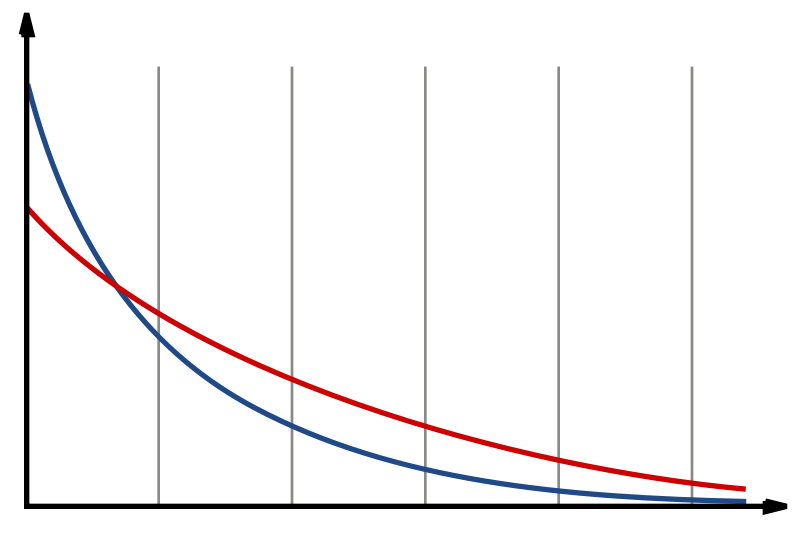
\includegraphics[width=0.5\textwidth]{LongTail.png}
  \caption{Una distribución de cola larga (roja) con una de cola no larga (azul).}
  \label{fig:longtailimg}
\end{figure}

\section{Objetivo}

\section{Alcance}